\chapter{Models and Associated Probes For Proton Spin Structure}
\label{ch:modeling_proton_spin}

With the advances made over the last half-century, we have come very close to
obtaining a complete model describing the world around us.  Rapid progress has
been made in the last 40 years in the understanding of the structure of the
nucleon. Protons and neutrons make up the majority of the mass in the visible
universe--therefore understanding their nature completely is of fundamental
importance to physics.

This thesis will discuss the experimental efforts of PHENIX to do something no
other experiment has done--utilize the production of $W$ Bosons as a direct
probe of proton spin. Before specifics of this are discussed, lets first put
proton spin into a larger context.

\section{Modeling the Proton Structure}

A constraint using particle accelerators to study any kind of nuclear
structure is that one does not ever get to directly look at the innards of a
proton, due to the phenomena of color confinement. 

This means that one must deal with the process of how partons (quarks, gluons)
fragment and decay after a proton proton collision in the final state.
Additionally, the scale variance of the fundamental forces plays an important
role.

The scale variance of the fundamental forces has large implications for the
strong nuclear force, represented by the coupling constant $\alpha_S$. This
constant scales with distance, and becomes highly non-perturbative at short
distances. Models must differentiate between perturbative and non-perturbative
processes. In perturbative models, the strategy is to write down a Hamiltonian
or Lagrangian to describe a system, and then obtain predictions from the model
by expanding in terms of a `small' parameter. Then, predictions from the leading
order, NLO, N$^2$LO or N$^3$LO are made and verified with data. Non perturbative
models often cannot write down all possible processes which contribute to the
overall Hamiltonian. Instead, non-perturbative models use structure functions
which take the form of global fits to experimental data. The models can then
make predictions through QCD evolution, which extrapolates the structure
functions to other energy scales, which again are probed experimentally.

The internal degrees of freedom of the proton, and the small scales involved
make models for the proton fall generally into non-perturbative regimes.  The
structure and distribution of partons and gluons in the nucleus is a
scale-dependent phenomena. That is to say, if one take measurements at a lower
energy, one may obtain a different distribution of partons and gluons at a
higher energy. This scale dependence requires many measurements to be taken
which probe different scales in order to properly constrain models for proton
structure. 

In order to properly model the non-perturbative structure of the proton,
Factorization Theorems are used. Factorization provides a means to
mathematically separate a probe interactions (such as electron-hadron scattering
in DIS) into perturbative and non-perturbative parts
(Figure~\ref{fig:disschematic}). Represented as a blob in such diagrams, the
non-perturbative aspect is the portion which is experimentally constrained.

\subsection{Structure Functions}
\label{sec:structure_functions}

Given that the proton itself has so far been shown to be a non-perturbative
object, the theoretical thrust is to create a probabilistic model for the proton
structure that can subsequently used to how two colliding protons interact and
generate particles. For each hadronic process, there is an associated structure
function. The variables defined to describe the kinematics of deep inelastic
scattering (Figure~\ref{fig:disschematic}) are :

\begin{gather}
  P \label{eq:P}\\
  Q^2 \equiv -q^2 \label{eq:big_q_sq}\\
  x \equiv { Q^2 \over {2P\cdot q} } \label{eq:x}
\end{gather}

{\noindent}$P$ is the total hadron momentum (in our case, the proton's
momentum), $Q^2$ is the momentum exchange between the proton and probe lepton,
and $x$ is the fraction of the total proton's momentum carried by the quark
scattering with the lepton.  $q$, in Equation~\ref{eq:x} is four-momentum
transferred from the lepton to the quark. \\

{\noindent}One can then write down structure functions in terms of these
variables, choosing the decomposition consistent with Lorentz Structure:

\begin{gather}
  F_1(x,Q^2) = {1 \over 2}\sum_f e_f^2 \left(q_f(x)+\bar{q}(x)\right)
  \label{eq:f1} \\
  F_2(x,Q^2) = 2xF_1(x,Q^2)\label{eq:f2}
\end{gather}

The subscript, $f$ refers to the quark flavors represented in the structure
functions, with $e_f$ referring to the charge of each quark being summed over
(i.e. ${\pm}{1\over3}$ or ${\pm}{2\over3}$). $q(x)$ refers to the parton
distribution function associated with each quark flavor. 

An integration over the momentum fraction, $x$ of Equation~\ref{eq:f2} and the
gluon structure function $g(x)$ yields the familiar `valence quark' structure of
the proton, i.e. two up-quarks and one down quark, with remaining quark flavors
$q_h$ summing to zero:

\begin{gather}
	\int_0^1 F_2(x,Q^2) + g(x) dx 
	= \int_0^1 
	\left(
		x\sum_f e_f^2 \left(q_f(x)+\bar{q}(x)\right) 
	\right) 
	+ g(x) dx \label{eq:f2_int_1} \\
	\int_0^1 \left(u(x)+\bar{u}(x) dx \right) dx = 2  \label{eq:up_quark_valence} \\
	\int_0^1 \left(d(x)+\bar{d}(x) dx \right) dx = 1  \label{eq:down_quark_valence} \\
	\int_0^1 \left(q_h(x)+\bar{q}_h(x) dx \right) dx = 0 \label{eq:other_quark_valence}
\end{gather}

The rest of the world data on $F_2(x,Q^2)$ is summarized in
Figure~\ref{fig:f2_world_data}

\begin{figure}[ht]
  \centering
  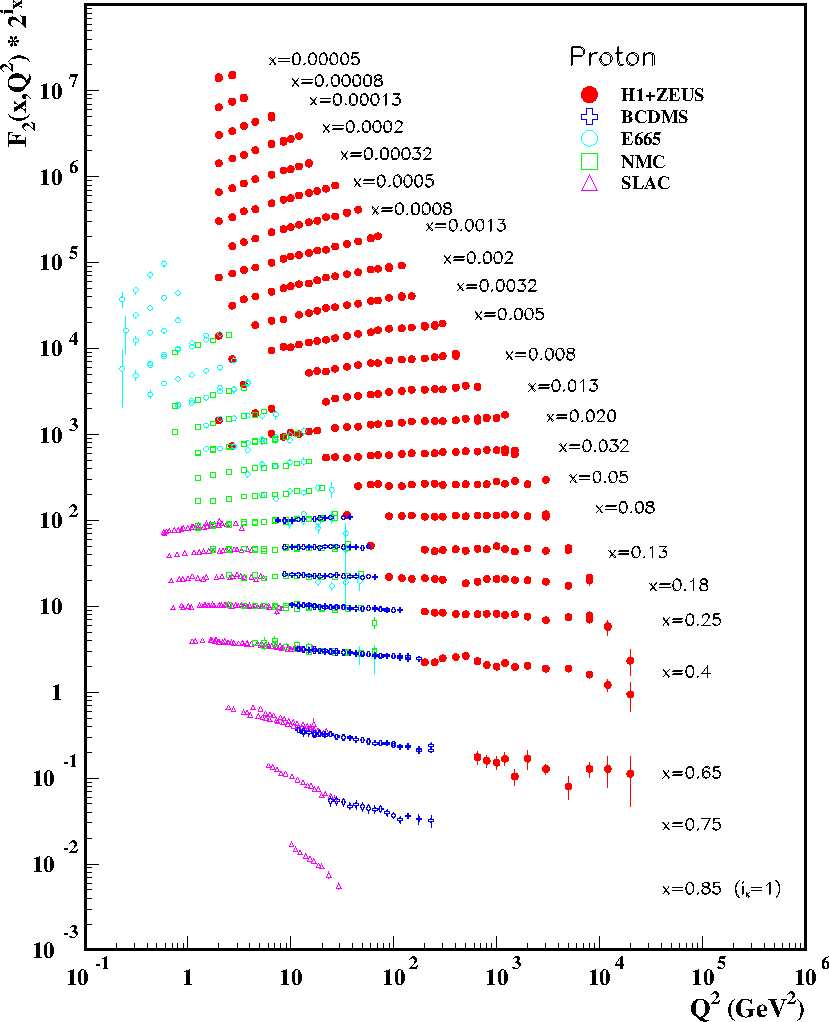
\includegraphics[width=\linewidth]{./figures/F2_structure_function.pdf}
  \caption{
    Shown: ``the proton structure function, $F_2^p$ measured in
		electromagnetic scattering experiments of electrons and positrons on
		protons'' from experiments including H1+Zeus, BCDMS, E665, NMC and
		SLAC~\cite{ReviewEidelman2012}
  }
  \label{fig:f2_world_data}
\end{figure}

\clearpage
\section{Parton Distribution Functions}
\label{sec:parton_distribution_functions}

From this dataset, the Parton Distribution Functions for any combination of $x$
and $Q^2$ may be extracted. Under this particular framework, DGLAP evolution
equations are used to evolve PDFs observed at one $Q^2$ to some other
$Q^2$~\cite{Altarelli2009}.

With QCD evolution, one can additionally undertake a global analysis, which
effectively puts a constraint on Parton Distribution functions using `evolved
projections' of $x$ and $Q^2$ into the kinematic range of the experimental
probes~\cite{Gal2014b}. 

The world data on proton structure can by evolved with the DGLAP
equations~\cite{Ellis1974} to generate parton distribution functions
representing the momentum fraction carried by various partons building up the
proton, the summary of this is shown in Figure~\ref{fig:unpolarized_pdf}. As expected--the PDF for $u$ is about twice as large as $d$
indicating the valence structure of the proton at high-x ($>0.1$). 

\begin{figure}[ht]
  \centering
  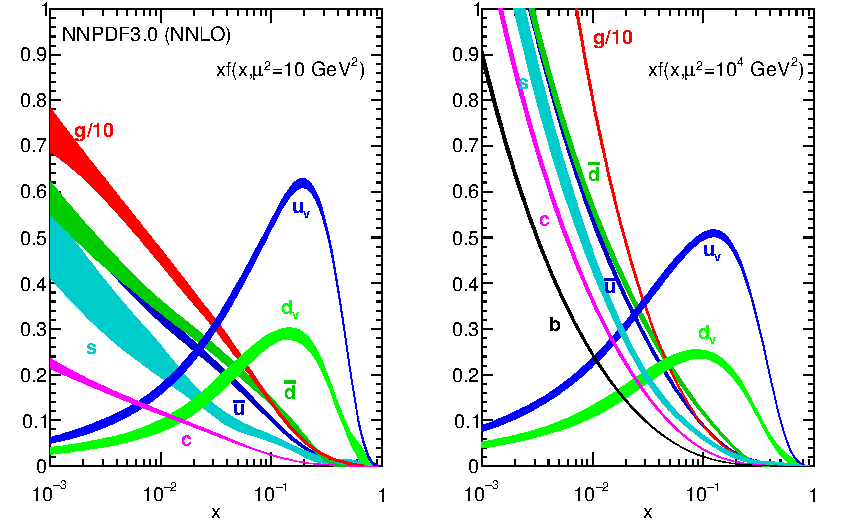
\includegraphics[width=0.7\linewidth]{./figures/unpolarized_pdfs.pdf}
  \caption{
    On the left is the NNPDF calculation of PDFs with world data (width is
    related to uncertainty) at 10 GeV, while 10 TeV is shown on the right. Note
    that at low $x$, the proton is dominated by
    gluons.~\cite{ReviewEidelman2012}.
  } 
  \label{fig:unpolarized_pdf}
\end{figure}

While DIS, and Semi-Inclusive Deep Inelastic Scattering have provided a wealth
of data on the proton's internal structure, RHIC data can be used to undertake a
complimentary analysis using hadron-hadron collisions, instead of hadron-lepton
collisions. A similar picture to DIS can be drawn of hadron-hadron interactions
to the DIS schematic, as seen in Figure~\ref{fig:hadron_inelastic_scattering}.

\begin{figure}[ht]
  \centering
	\begin{subfigure}{0.5\textwidth}
		\centering
		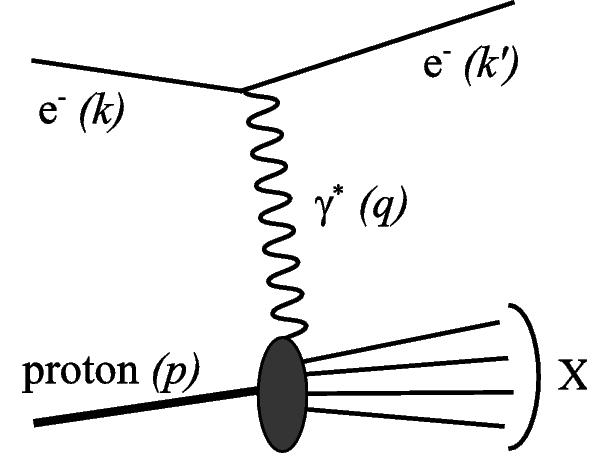
\includegraphics[width=\textwidth]{./figures/deep_inelastic_basic.png}
    \caption{Leptonic Deep Inelastic Scattering}
		\label{fig:dis}
	\end{subfigure}%
	\begin{subfigure}{0.5\textwidth}
		\centering
		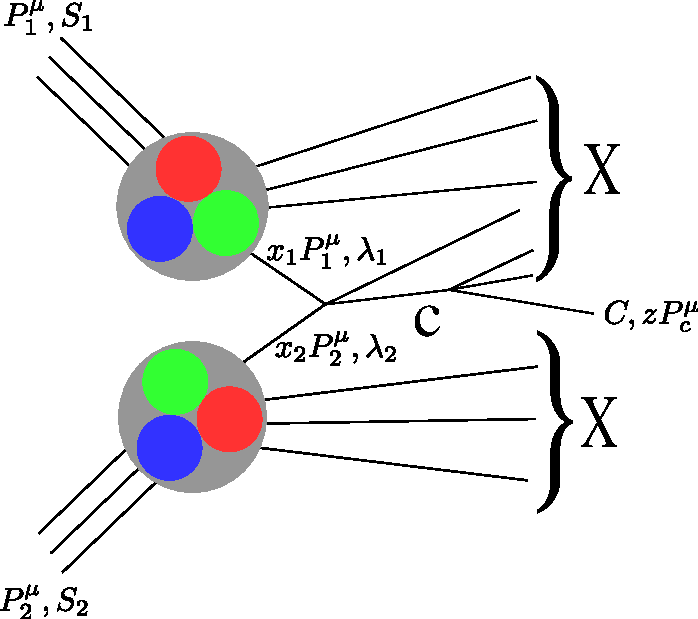
\includegraphics[width=\textwidth]{./figures/hadron_inlastic_scattering.pdf}
    \caption{Hadronic Inelastic Scattering}
    \label{fig:his}
	\end{subfigure}
  \caption{
    Deep Inelastic Scattering Process (Panel (a)) alongside Hadron-Hadron
    inelastic scattering (Panel (b)). In hadron inelastic scattering, one may
    try to select initial state with scattering between arbitrary partons in
    order to probe various proton structures.
  }
  \label{fig:hadron_inelastic_scattering}
\end{figure}

Hadron-Hadron scattering can be a useful means to determine PDFs experimentally,
but often intermediate states are not known and it is difficult to isolate a
single PDF. Hadron-hadron scattering experiments provide an excellent source of
data to constrain gluon PDFs.

\subsection{Polarized Parton Distribution Functions}
\label{sec:polarized_parton_distribution_functions}

Polarized parton distributions are measured with the same methods discussed
above--except the beam and/or target in the scattering formalism are
spin-polarized. We can similarly write down the structure functions for
polarized protons, in the same manner as $F_1$ and $F_2$:

\begin{equation}
  g_1 = {1 \over 2}\sum_q e_q^2(q^+(x)-q^-(x)) 
  = {1 \over 2} \sum_q e^2_q\Delta q(x)
  \label{eq:g1}
\end{equation}

Here, $e_q$ is the charge of the quark-flavor (i.e., $1/3e$, $2/3e$), with the
sum taken over all quark/anti-quark flavors. The $q$ terms refer to the number
density of each particularly quark flavor associated with the ``+'' or ``-''
quark spin orientation (relative to the struck hadron), such that ``+'' refers
to a parallel spin and ``-'' refers to an anti-parallel spin. $g_1$ describes
the longitudinal spin polarization of the nucleus, while $g_2$ describes the
transverse spin polarization of the nucleus. A knowledge of both longitudinal
and transverse spin structure is necessary for a complete understanding of the
three-dimensional structure of the proton.

The experimental tool for measurement of the spin structure of the proton is the
`spin asymmetry'. The spin asymmetry is defined in terms of scattering
cross-sections, therefore one may experimentally determine these cross sections,
or calculate these cross sections from models. In particular, the asymmetry is
directly proportional to the structure functions describing the proton:

\begin{align}
  A(x,Q^2) &= 
  {{\sigma^+-\sigma^-}\over{\sigma^++\sigma^-}} \label{eq:al_simple} \\
           &\equiv 
  {{g_1(x,Q^2)}\over{F_1(x,Q^2)}} \label{eq:al_structure}
\end{align}

{\noindent}With our knowledge of $F_1$ from fits to the world's data
(Fig.~\ref{fig:f2_world_data}), the asymmetry may provide a direct measurement
of $g_1$ ~\cite{DeFlorian2009}. With the discovery that the proton's spin is not
entirely carried by the valence quarks, one may construct additional
spin-dependent parton distribution functions, and design experiments to measure
and constrain them. Current knowledge of parton distribution functions is
summarized in Figure~\ref{fig:polarized_pdfs_1} and \ref{fig:polarized_pdfs_2}.

\begin{figure}[ht]
  \centering
  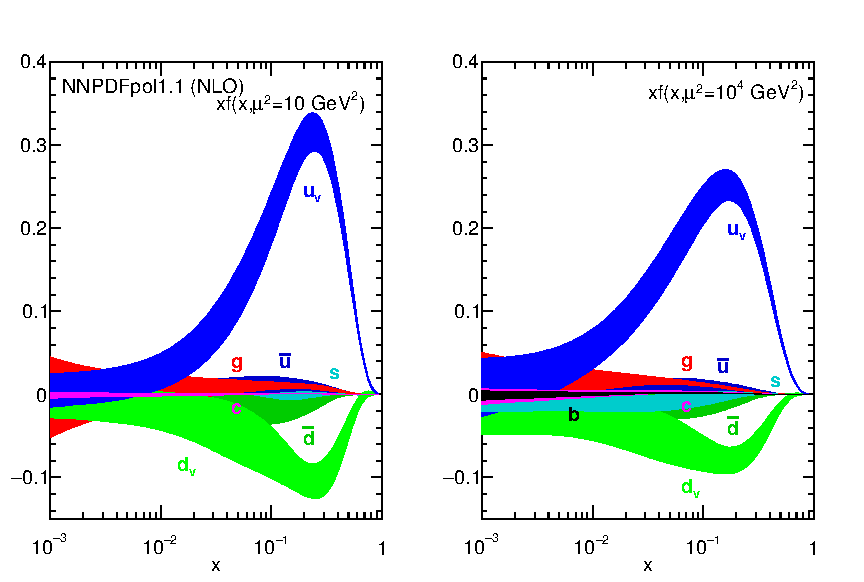
\includegraphics[width=0.7\linewidth]{./figures/polarized_pdfs.pdf}
  \caption{
    World data used to generate fits to predict the parton distribution
    functions of various quark flavors in the proton at 10 GeV (left) and 10
    TeV (right)~\cite{ReviewEidelman2012}
  }
  \label{fig:polarized_pdfs_1}
\end{figure}

\begin{figure}[ht]
  \centering
  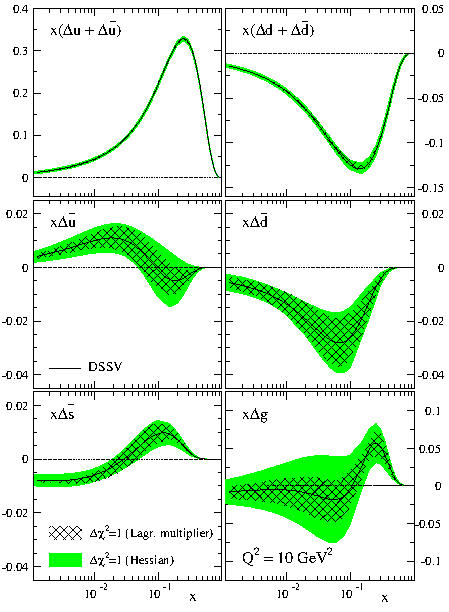
\includegraphics[width=0.8\linewidth]{./figures/polarized_pdfs_dssv.pdf}
  \caption{
    PDFs for polarized parton distribution functions shown at 10 GeV for quarks,
    anti-quarks, and gluons in the proton. The uncertainties for the gluon and
    anti-quark PDFs are quite large, warranting experimental
    investigation~\cite{DeFlorian2009}.
  }
  \label{fig:polarized_pdfs_2}
\end{figure}

\clearpage
\section{Proton Spin Decomposition with the Ellis-Jeffe Sum Rule }

The spin contribution of the proton may be written as a sum of the various
spin contributions using the polarized parton distribution functions. The
particulars of the decomposition vary with the chosen gauge. Ellis-Jeffe
produced a gauge invariant decomposition:

{\noindent}Gauge invariant Ellis-Jeffe
\begin{equation}
  \braket{P,{1\over2}|\hat{J_z}|P,{1\over2}}  
 = {1\over2} = {{1\over2}\Delta \Sigma +L_q+J_g}
\label{eq:ellis_jeffe_sum}
\end{equation}

{\noindent}and another, intuitive decomposition, in the infinite momentum gauge:
\begin{equation}
  \braket{P,{1\over2}|\hat{J_z}|P,{1\over2}}  
  = {1\over2} = {{1\over2}\Delta \Sigma +L_q+\Delta g + L_g}
  \label{eq:infmom_ellis_jeffe_sum}
\end{equation}

{\noindent}The quark helicity distribution is subdivided into its flavor
structure:
\begin{equation}
  {\Delta \Sigma} =
  {
    (\Delta u+\Delta \bar{u})
    +(\Delta d + \Delta \bar{d})
    +(\Delta s + \Delta \bar{s})
  }
  \label{eq:quark_spin_decomposition}
\end{equation}

{\noindent}As discussed earlier, there is a large uncertainty in the
contribution of the anti-quarks to the proton spin which this work seeks to
constrain.

\section{The Spin Asymmetry: An Experimental Probe }

The spin asymmetry is an important experimental probe into the longitudinal spin
structure function, $g_1$ from which one derives polarized parton distribution
functions. At RHIC, hadron inelastic scattering is used to generate events from
which asymmetries for various final-states are measured. The probes available at
RHIC via hadronic deep inelastic scattering are summarized in
Figure~\ref{fig:spin_probes_masterspin}.

\begin{figure}[ht]
  \centering
  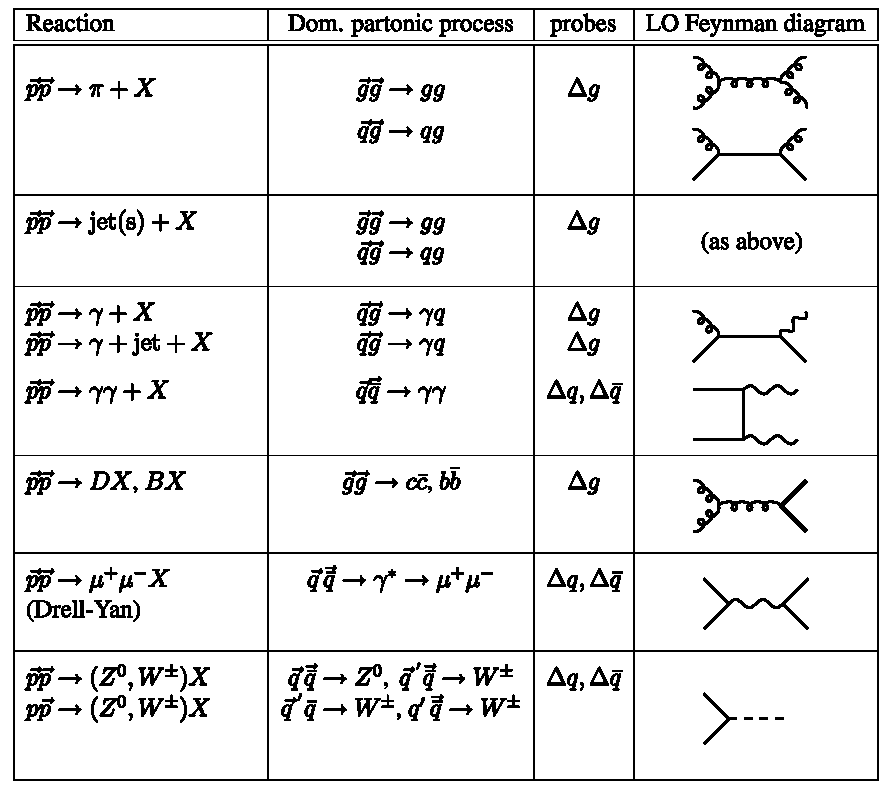
\includegraphics[width=\linewidth]{./figures/spin_probes.pdf}
  \caption{
    A summary of the various probes for longitudinally polarized protons. The
    \textbf{``Reaction''} column summarizes the reaction observed
    experimentally.  The \textbf{``Dom. partonic process''} column describes the
    dominant process at the partonic level. The \textbf{``probes''} column shows
    which proton spin structure can be measured with the reaction. Finally, the
    leading order Feynman diagram for the partonic process is
    drawn~\cite{Aidala2005}.
  }
  \label{fig:spin_probes_masterspin}

\end{figure}

One potential pit-fall of using hadronic initial states in spin measurements is
the issue of fragmentation. Fragmentation complicates the process of determining
the initial state interaction and measuring the correct final state. For
example, consider measuring a photonic decay from a final state. A $pi^0$ can
produced as part of a specific initial state of interest, however $\pi^0$'s can
be produced in a vast array of fragmentation processes, and all of them can
decay to photons. It can be hard to isolate the parent interaction which
produces the particles of interest. 

Consider as a contrast, the production of the $W$. The $W$ decay offers a
clean probe free of fragmentation, useful for studying the polarization of
anti-quark parton distribution functions. Specifically, due to the parity
violating nature of the $W$ decay, $W$'s  will only couple to left handed
particles and right handed anti-particles. Consider too the relativistic
neutrino resulting from the $W$ decay. Due to this, interactions producing a $W$
boson necessarily have the helicity state in the initial state fixed. This makes
the $W$ boson an attractive candidate for studying the sea-quark polarization of
the proton.

While all weak processes are mediated by the W/Z boson, real $W$ production from
$q+\bar{q}$ interactions produce a clear Jacobean peak at central rapidities at
the 510 GeV $\sqrt{s}$ collision energy of interest (at PHENIX), and
additionally can be identified at forward rapidities using statistical methods
discussed in Chapter~\ref{ch:feature_engineering}.

\clearpage
\section{$W$ Production}

Though the $W$ can be created in collisions with the right ingredients and
correct energy, the $W$ decays that PHENIX seeks to measure are very special.
The conditions of collision at the PHENIX interaction region provides enough
energy to create real $W$ Bosons from direct parton-parton interactions between
protons. However, the energy is not sufficiently high enough to produce real $W$
Bosons from secondary decay processes in amounts which would significantly
dilute the primary source.

The standard model tells us that W production occurs through a pure vector-axial
interaction. This implies that the helicity of the parents particles--in
particular $u+\bar{d}\rightarrow W^+$ and $\bar{u}+d\rightarrow W^-$ are fixed,
due to the relativistic final state neutrino, and the maximal parity violating
nature of the interaction. To visualize the leading order of W production, with
regards to the quark-sea element being probed, the leading order diagrams for
the interaction are shown in
Figure~\ref{fig:w_probe_leading_order}~\cite{Aidala2005}

We probe the polarized parton distribution functions representing quarks and
anti-quarks by measuring the asymmetry of the decay products of the $W$,
with respect to the helicities of the protons in the initial state. $\Delta q$,
the polarized parton distribution function representing the quark contribution
to proton spin Equation~\ref{eq:ellis_jeffe_sum} can be subdivided into
further quark PDFs, Equation~\ref{eq:quark_spin_decomposition}. The $W$ boson
decay provides a unique glimpse into specifically the anti-quark polarized
parton distribution functions.

\begin{figure}[ht]
  \centering
  \begin{subfigure}[b]{\textwidth}
    \centering
    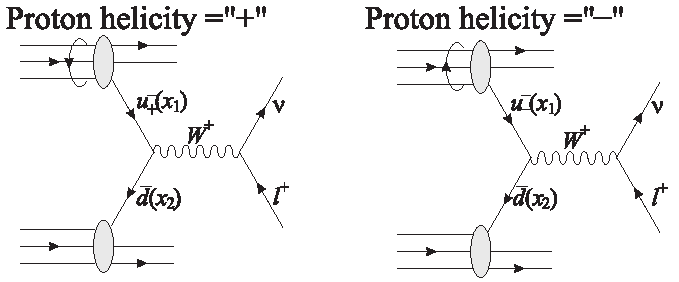
\includegraphics[width=0.8\linewidth]{./figures/w_plus_u_probe.pdf}
    \caption{
      Probe for $\Delta u$ at lowest order.
    }
    \label{fig:u_probe}
  \end{subfigure}
  \begin{subfigure}[t]{\textwidth}
    \centering
    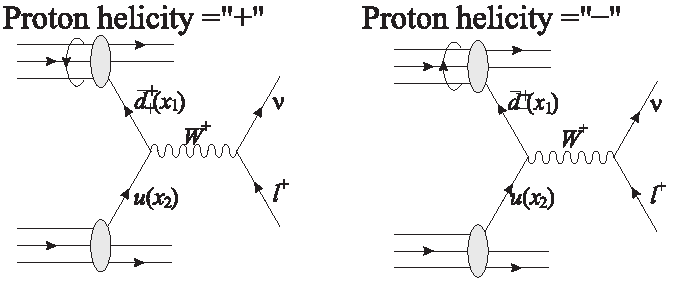
\includegraphics[width=0.8\linewidth]{./figures/w_plus_dbar_probe.pdf}
    \caption{
      Probe for $\Delta\bar{d}$ at lowest order
    }
    \label{fig:dbar_probe}
  \end{subfigure}
  \caption{
    Real $W^+$ production as produced at PHENIX. The helicity of the initial
    state fixes the helicity of the partonic participants due to the
    relativistic final state of the neutrino + the handedness of the $W$.  $x_1$
    and $x_2$ are the momentum fractions of the quarks participating from the
    participant partons~\cite{Aidala2005}. 
  }
  \label{fig:w_probe_leading_order}
\end{figure}

PHENIX collides polarized protons, but the polarization of one participant
proton can be effectively ignored by summing over all polarization states for
one of the two protons. With this assumption, one may construct a single spin
asymmetry for colliding protons by counting difference in the number of
positively and negatively polarized $W$'s produced in collisions, scaled by the
total production:

\begin{equation}
  {{A_L}^W} =
  {{{1}\over{P}}\times{{N_{-}(W)-N_{+}(W)}\over{{N_{-}(W)+N_{+}(W)}}} }
  \label{eq:w_production_asymmetry}
\end{equation}

This extraction of this experimental probe is discussed in
Chapter~\ref{ch:feature_engineering}.

As seen earlier, in Section~\ref{sec:polarized_parton_distribution_functions},
one may write an asymmetry in terms of the scattering cross section for the
process responsible for particle yields. These cross-sections were shown to be
written in terms of polarized parton distribution functions. The full expression
of the theoretical asymmetries for this process are written in terms of the
parton distribution functions, with implicit integration over $x_1$ and $x_2$.

For $W^+$ and $u$:
\begin{equation}
  {A_L^{W^+}} = 
  {
    {u_-^-(x_1)\bar{d}(x_2)-u_+^-(x_1)\bar{d}(x_2)}
    \over
    {u_-^-(x_1)\bar{d}(x_2)-u_+^-(x_1)\bar{d}(x_2)}
  }  
  \label{eq:al_u_full}
\end{equation}

For $W^+$ and $\bar{d}$
\begin{equation}
  {A_L^{W^+}} = 
  {
    {\bar{d}_-^+(x_1)u(x_2)-\bar{d}_+^+(x_1)u(x_2)}
    \over
    {\bar{d}_-^+(x_1)u(x_2)+\bar{d}_+^+(x_1)u(x_2)}
  }  
  \label{eq:al_dbar_full}
\end{equation}

{\noindent}Observationally, a superposition of \ref{eq:al_u_full} is seen and
\ref{eq:al_dbar_full}, which is expressed in
Equation~\ref{eq:al_superposition_pos}:

\begin{equation}
  {A_L^{W^+}} = 
  {
    {
      \Delta u(x_1)\bar{d}(x_2)-\Delta \bar{d}(x_1)u(x_2)
    }
    \over
    {
      u(x_1)\bar d(x_2)+\bar(d)(x_1)u(x_2)
    }
  }
  \label{eq:al_superposition_pos}
\end{equation}

{\noindent}For the case of $W^-$, we observe $\bar{d}$ and $u$. For $W^-$ and $d$:
\begin{equation}
  {A_L^{W^+}} = 
  {
    {d_-^-(x_1)\bar{u}(x_2)-d_+^-(x_1)\bar{u}(x_2)}
    \over
    {d_-^-(x_1)\bar{u}(x_2)-d_+^-(x_1)\bar{u}(x_2)}
  }  
  \label{eq:al_d_full}
\end{equation}

{\noindent}For $W^-$ and $\bar{u}$
\begin{equation}
  {A_L^{W^+}} = 
  {
    {\bar{u}_-^+(x_1)d(x_2)-\bar{u}_+^+(x_1)d(x_2)}
    \over
    {\bar{u}_-^+(x_1)d(x_2)+\bar{u}_+^+(x_1)d(x_2)}
  }  
  \label{eq:al_ubar_full}
\end{equation}

{\noindent}Observationally, the superposition of \ref{eq:al_d_full} and
\ref{eq:al_ubar_full} is measured:
Equation~\ref{eq:al_superposition_neg}:

\begin{equation}
  {A_L^{W^-}} = 
  {
    {
      \Delta d(x_1)\bar{u}(x_2)-\Delta \bar{u}(x_1)d(x_2)
    }
    \over
    {
      d(x_1)\bar u(x_2)+\bar(u)(x_1)d(x_2)
    }
  }
  \label{eq:al_superposition_neg}
\end{equation}

{\noindent}Kinematics of the collision can simplify the equations even
further~\cite{Aidala2005}. Concretely, this is shown via integration over the
momentum fractions, $x_1$ and $x_2$, explicitly writing the W decay in terms of
the scattering cross section for polarized proton collisions (a derivation
reproduced from \cite{Oide2012}):

\begin{multline}
  {
    d\sigma
    \left(
      p^{\Rightarrow}+p\rightarrow W^+\rightarrow \ell+\nu_{\ell}
    \right)
  } 
  = \\
  {
    {K\over3}\int dx_1dx_2\sum_{i,j}
    \left(
    q_{i-}^\Rightarrow(x_1)\bar{q}_{j+}(x_2) +
    \bar{q}_{j+}^\Rightarrow(x_1)q_{i-}(x_2)
    \right)
  }  \\
  \times
  {
    d\hat{\sigma}(q_i+\bar{q}_j\rightarrow W^+\rightarrow \ell^+ + \nu_{\ell})
  }
\end{multline}

{\noindent}Similarly, we may write the interaction cross-section for the
opposite helicity in the initial state:

\begin{multline}
  {
    d\sigma
    \left(
      p^{\Leftarrow}+p\rightarrow W^+\rightarrow \ell+\nu_{\ell}
    \right)
  } 
  = \\
  {
    {K\over3}\int dx_1dx_2\sum_{i,j}
    \left(
    q_{i-}^\Leftarrow(x_1)\bar{q}_{j+}(x_2) +
    \bar{q}_{j+}^\Leftarrow(x_1)q_{i-}(x_2)
    \right)
  }  \\
  \times
  {
    d\hat{\sigma}(q_i+\bar{q}_j\rightarrow W^+\rightarrow \ell^+ + \nu_{\ell})
  }
\end{multline}

{\noindent}Assuming massless quarks, the helicity state of the quarks becomes
identical to the chirality state. Then, substitute in the definition for
polarized parton distribution functions $\Delta q \equiv q_{+}^{\Rightarrow} -
q_{-}^{\Rightarrow}$, and sum over quark flavors. Strange quarks do not
contribute:

\begin{align}\label{eq:al_theory_quarks}
  {
    A_L
    \left(
      p^{\Rightarrow}+p\rightarrow W^+ \rightarrow \ell^+ +\nu_{\ell}
    \right)
  } &=  
  {
    {
      \int dx_1 dx_2 \sum_{i,j}
      \left(
        -\Delta q_i(x_1)\bar{q}_j(x_2)
        +\Delta \bar{q}_j(x_1)q_i(x_2)
      \right)\cdot d \hat{\sigma}
    }
    \over
    {
      \int dx_1 dx_2
      \sum_{i,j}(q_i(x_1)\bar{q}_j(x_2)+\bar{q}_j(x_1)q_i(x_2))\cdot d\hat{\sigma}
    }
 }\\
 & \approx  \nonumber
 {
   {
      \int dx_1 dx_2 
      \left(
        -\Delta u(x_1)\bar{d}(x_2)
        +\Delta \bar{d}(x_1)u(x_2)
      \right)\cdot d \hat{\sigma}
   }
   \over
   {
      \int dx_1 dx_2 (u(x_1)\bar{d}(x_2)+\bar{d}_j(x_1)u(x_2))\cdot d\hat{\sigma}
   }
 }
\end{align}

{\noindent}Since we have restricted ourselves to only the case for $u\bar{d}$,
$A_L^{W+}$ is observed. Equation~\ref{eq:al_theory_quarks} is rewritten to
reflect its rapidity dependence:

\begin{equation}
  {A_L^{W+}(y_{\ell})} = 
  {
    {
     \int dx_1 dx_2 
     \left(
       -\Delta u(x_1)\bar{d}(x_2)(1-cos\hat{\theta})^2
       +\Delta \bar{d}(x_1)u(x_2)(1+cos\hat{\theta})^2
     \right)
    }
    \over
    {
       \int dx_1 dx_2 
       \left(
       (u(x_1)\bar{d}(x_2)   (1-cos\hat{\theta})^2
      +\bar{d}_j(x_1)u(x_2)) (1+cos\hat{\theta})^2
        \right)
    }
  }
  \label{eq:al_w_pos_rapidity_dependance}
\end{equation}

{\noindent}In this case, we follow the notational convention of~\cite{Oide2012}
and $\hat{\theta}$ in terms of the angle between the direction of momentum of
the polarized proton and the lepton in the center of mass frame. Therefore,
decoupling of $Delta\bar{u}$ and $\Delta\bar{d}$ is achieved at forward or
backward rapidity.

{\noindent}We may write $A_L^{W-}(y_{\ell})$ similarly:

\begin{equation}
  {A_L^{W-}(y_{\ell})} = 
  {
    {
     \int dx_1 dx_2 
     \left(
       -\Delta \bar{u}(x_1)d(x_2)(1-cos\hat{\theta})^2
       +\Delta d(x_1)\bar{u}(x_2)(1+cos\hat{\theta})^2
     \right)
    }
    \over
    {
       \int dx_1 dx_2 
       \left(
         (\bar{u}(x_1)d(x_2)   (1-cos\hat{\theta})^2
         +d_j(x_1)\bar{u}(x_2)) (1+cos\hat{\theta})^2
        \right)
    }
  }
  \label{eq:al_w_neg_rapidity_dependance}
\end{equation}
\clearpage

With an understanding of the $W$ process and ability to probe the helicity
dependent parton distribution functions, the remaining challenge is to use RHIC
and PHENIX to record this data set, discussed next!
